\chapter{Исследовательский раздел}

В данном разделе проводится исследование характеристик созданной базы данных. А именно исследование времени поиска и создания узла. Перед проведением исследования указываются технические характеристики устройства, на котором данное исследование проводится. На основе полученных результатов делается вывод о том, как на исследуемые характеристики системы зависят от количества существующих узлов в базе данных.

\section{Технические характеристики}

При проведении исследования какой-либо системы важно знать какими характеристиками обладает устройство, на котором проводятся измерения, так как численные результаты могут изменяться от устройства к устройству.
Технические характеристики устройства, на котором выполнялись измерения:

\begin{enumerate}
	\item операционная система: Windows 10 Pro Версия 21H1 x64~\cite{oswindows};
	\item оперативная память: 8 ГБ;
	\item процессор: 2,4 ГГц 4-ядерный процессор Intel Core i5-1135G7\cite{intel}.
\end{enumerate}

Во время замеров ноутбук был включен в сеть электропитания, нагружен
только самим приложением.

\section{Анализ времени поиска узла по связям}

В процессе использования приложения пациент будет составлять предложения из слов, возможна ситуация в которой необходимо соединить 2 слова неким другим словом, связанным с начальными.
В такой ситуации требуется как можно быстрее находить все варианты недостающего слова в базе данных.

Исследование проводится для получения зависимости времени получения ответа от количества узлов в базе данных.

В таблице \ref{table_measuring_rs1} и на графике \ref{rs1} представлены результаты замеров времени при разном количестве узлов.

\newcolumntype{d}[1]{D{.}{.}{-1}}

\begin{table}[h!]
	\begin{center}
		\begin{threeparttable}
			\captionsetup{justification=raggedright,singlelinecheck=off}
			\caption{Замеры времени поиска узла по двум <<соседним>>}
			\label{table_measuring_rs1}
			\begin{tabular}{|c|d{4.3}|}
				\hline
				Количество узлов & \multicolumn{1}{c|}{\text{Время (мс)}} \\
				\hline
				15 & 1 \\
				\hline
				25 & 2 \\
				\hline
				40 & 3.5\\
				\hline
				50 & 3.5\\
				\hline
				70 & 5.5\\
				\hline
				90 & 7\\
				\hline
				100 & 8\\
				\hline
				115 & 8.5\\
				\hline
				135 & 9\\
				\hline
			\end{tabular}
		\end{threeparttable}
	\end{center}
\end{table}

\begin{figure}[ht!]\centering
	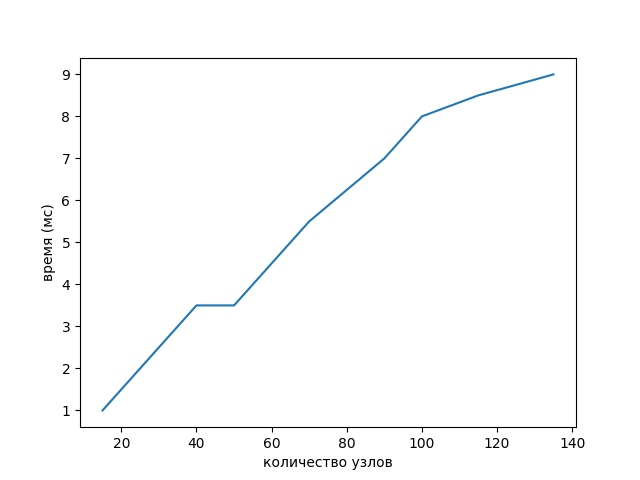
\includegraphics[scale=0.8]{rs1}
	\caption{Замеры времени поиска узла по двум <<соседним>>}
	\label{rs1}
\end{figure}

По результатам замеров видно, что время линейно зависит от количества узлов в базе данных.

\pagebreak

\section{Анализ времени добавления узла}

В процессе развития пациента в базу данных будут добавляться новые слова. 

Исследование проводится для получения зависимости времени добавления узла от количества уже имеющихся узлов в базе.

В таблице \ref{table_measuring_rs2} и на графике \ref{rs1} представлены результаты замеров времени при разном количестве узлов.

\begin{table}[h!]
	\begin{center}
		\begin{threeparttable}
			\captionsetup{justification=raggedright,singlelinecheck=off}
			\caption{Выборка из замеро времени добавления узла}
			\label{table_measuring_rs2}
			\begin{tabular}{|c|d{4.3}|}
				\hline
				Количество узлов & \multicolumn{1}{c|}{\text{Время (мс)}} \\
\hline
50 & 2.8 \\
\hline
100 & 2.0 \\
\hline
150 & 1.0 \\
\hline
200 & 2.5 \\
\hline
250 & 3.8 \\
\hline
300 & 3.7 \\
\hline
350 & 3.4 \\
\hline
400 & 5.5 \\
\hline
450 & 3.7 \\
\hline
500 & 3.1 \\
\hline
			\end{tabular}
		\end{threeparttable}
	\end{center}
\end{table}

\begin{figure}[ht!]\centering
	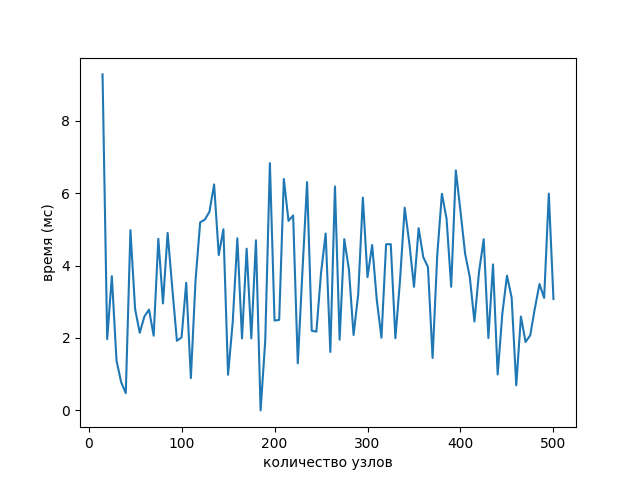
\includegraphics[scale=0.67]{rs2}
	\caption{Замеры времени добавления узла}
	\label{rs2}
\end{figure}

\clearpage

По результатам замеров видно, что время создания нового узла не зависит от времени.

\section*{Вывод}

В данном разделе были представлены технические характеристики устройства на котором проводились измерения. В процессе исследования было обнаружено, что время поиска узла по двум <<соседним>> линейно завит от количества узлов в базе данных. Однако также замечено, что время создания узла не зависит от общего количества узлов.
